\section{Energy integration}


Nasibeh use cetow for heat puming solutions and st fons for large scale integration and combined heat and power production. We have to use neutralised values (i.e. we start with 100 unit and end up with 46.


Converting energy resources into useful energy, exergy efficiency, heat pumping and combined heat and power => examples from the papers of Nasibeh

adding a citation \cite{Pouransari_2014}

testing equations
\begin{equation}
min \, obj= \frac{things_{good}}{things_{bad}} \forall things\\
\text{subject to}  \\
things_{bad}\ge necessary\,\, level \cup unnecessary \, level
\end{equation}

**************

\subsection{Caste study I: Energy integration technologies}

\begin{figure}[h]
        \begin{center}
        \begin{tabular}{cc}
        \subfloat[Composite Curve]{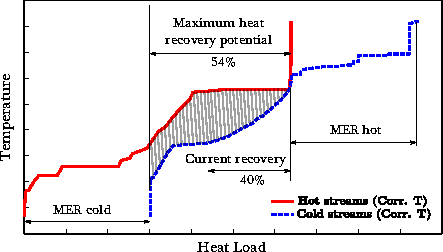
\includegraphics [height=4.3cm]{figures/EnergyIntegration/figMERcc.pdf}} & 
        \subfloat[Grand Composite Curve]{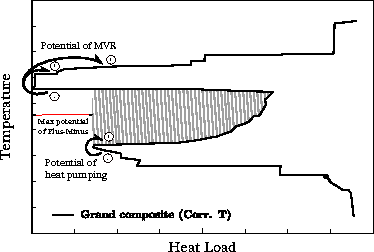
\includegraphics [height=4.3cm]{figures/EnergyIntegration/figMERgcc.pdf}}
        \end{tabular}
        \caption{Pinch analysis step results}
        \label{fig1:mer}
        \end{center}
        \end{figure}
        
